\documentclass[12pt]{article}
\usepackage[utf8]{inputenc}
\usepackage{amsmath}
\usepackage{graphicx}
\usepackage{float}
\usepackage[margin=1in]{geometry}
%%
\usepackage{color}
\usepackage{lineno}
\renewcommand\thelinenumber{\color{cyan}\arabic{linenumber}}
%%
\setlength{\parskip}{1em}
\renewcommand{\baselinestretch}{1.5}
\newcommand\dbyd[2]{\frac{\mathrm d{#1}}{\mathrm d{#2}}}
\newcommand\dsided[2]{{\mathrm d{#1}}/{\mathrm d{#2}}}
\newcommand{\R}{\mathcal{R}}
\title{Intentional infection as a method of\\population-level disease control}
\author{Roger Zhang}
\date{June 16th 2018}
\usepackage{color}
\newcommand{\david}[1]{\textcolor{blue}{$\langle${\slshape{\bfseries David:} #1 }$\rangle$}}
\newcommand{\roger}[1]{\textcolor{red}{$\langle${\slshape{\bfseries Roger:} #1 }$\rangle$}}
\usepackage[colorlinks=true,linkcolor=blue]{hyperref}
\newcommand{\pmV}{p_{V}}
\newcommand{\pmI}{p_{I}}


\begin{document}
\linenumbers
\maketitle
\begin{abstract}
In this paper, we study the possible advantages of intentional infection, as a method of population-level disease control. Intentional infection is a generalization of variolation, which was invented in 15th century, and widely used around the world in 17th and 18th century. People believed that by variolation, a mild but protective infection would result, which give them a higher chance of survival compared to being naturally infected. This paper aims to provide mathematical models which describes the dynamics of infected classes, when intentional infection is introduced on a population level, and perform predictions based on the models.
\end{abstract}
\clearpage
\tableofcontents
\clearpage
\section{Introduction}
Disease control has drawn people's attention since the early age of human civilization. Other than curing diseases by medication, people have also discovered and attempted vast range of method for disease prevention. In this era, people have vaccination as a primary method to protect the population. Before vaccination becomes a developed technology, people had limited power when encountering fatal diseases such as smallpox.

A technology called variolation was invented as an attempt to contain smallpox. The earliest record of such method can be found in 15th century's ancient Chinese documentation. It is a method used to immunize individuals against smallpox, with materials taken from other smallpox patient or recently variolated individuals. People have found that, by variolation, a mild, but protective infection will likely occur, as a result, variolated individuals die much less often.

More generally speaking, similar method may be applied to other diseases for disease control as well. Fundamentally speaking, variolation is an example of intentional infection, since individuals are deliberately exposed living virus. Although an individual benefits from intentional infection when there is threat of being transmitted with fatal disease, people did not understand whether intentional infection can also bring positive effect when applied on a population level. 

Similar to vaccination, there are different strategies for variolation. One example of strategy is to intentional infect newborn individuals. In fact, newborn infection does not mean instant infection when people are born, but rather after their maternal immunity wanes. Another strategy we consider in this paper is to intentionally infect susceptible individuals in the population, at a certain rate. 

\section{Models: Intentional infect proportion of susceptible}
\subsection{Model: Modification to SIR model}
\subsubsection{System of differential equations}
We begin our analysis by modifying SIR model. Our first strategy is to intentionally infect newborn individuals, with a certain proportion.  The following assumptions are made to simplify the model to start with:
\begin{itemize}
\item No difference between intentionally infected and naturally infected individuals.
\item No disease induced mortality(Addition of disease induced mortality will be ).
\item Birth and natural death rate are the same(total population $N$ remains constant).
\item The latent period(time from infection to becoming infectious) is short enough to be ignored.
\item All susceptible individuals are equally likely to be infected, and all infected individuals are equally infectious.
\end{itemize}
Equipped with the assumptions above, we now setup our system of differential equations.

Just like in SIR model, $S$, $I$ and $R$ represent the proportion of susceptible, infected and recovered with respect to total population.
\begin{equation}\label{1}
\begin{split}
\dbyd{S}{t}&=\mu(1-p)- \beta SI-\mu S \,,\\
\dbyd{I}{t}&=\beta SI+\mu p-\gamma I -\mu I\,,\\
\dbyd{R}{t}&=\gamma I-\mu R\,.
\end{split}
\end{equation}
Here, $\beta$ is the transmission rate, $\gamma$ is the recovery rate,
$\mu$ is the \emph{per capita} rate of birth and death, $p$ is the
proportion of newborns that are intentionally infected.

We non-dimensionalize \autoref{1} by scaling time, by
\begin{equation}
\tau=(\gamma+\mu)t \,,
\end{equation}
so the time unit now is ``mean time infected".

The dimensionless system is:
\begin{subequations}\label{3}
\begin{align}
\dbyd{S}{\tau}&=\epsilon(1-p)- \R_0  SI-\epsilon S \,,\\
\dbyd{I}{\tau}&=\R_0 SI+\epsilon p-I \,,
\end{align}
\end{subequations}
where $\epsilon=\frac{\mu}{\gamma+\mu}$, $\R_0=\frac{\beta}{\gamma+\mu}$.

We are not considering $\dbyd{R}{\tau}$ since it does not impact the dynamics of $S$ and $I$, and we do not need to track the proportion of recovered individuals in this model.
\subsubsection{Equilibria}
By letting \autoref{3} equal to 0, we solve for equilibria. The only equilibrium for this model is,
\begin{subequations}
\begin{align}
\hat{S} &=\frac{1}{\R_0}-\frac{2p}{(\R_0 -1)+ \sqrt{(\R_0-1)^2+4\R_0 p}}\,, \label{Shat1}\\
\hat{I} &= \frac{\epsilon(\R_0 -1)+ \epsilon \sqrt{(\R_0-1)^2+4\R_0
    p}}{2\R_0}\,.\label{Ihat1}
\end{align}
\end{subequations}

Notice, \autoref{Ihat1} does not return 0 for any $p$ value between 0 and 1, meaning there is always infected individuals present in the population. Therefore, we can claim that this is not a disease free equilibrium. It follows that the equilibrium above is an endemic equilibrium (EE).

We would like to know if the EE is stable, therefore we need the Jacobian matrix of \autoref{3}. The Jacobian is, 
\begin{equation}
\mathcal{J} =
\begin{bmatrix}
    \ -\R_0 I-\epsilon       & -\R_0 S \\
    \ \R_0 I       & \R_0 S-1 \\
\end{bmatrix} \,.
\end{equation}

Now for simplicity, let 
\begin{equation}\label{E:}
K = (\R_0-1)+ \sqrt{(\R_0-1)^2+4\R_0 p} \,.
\end{equation}

For the purpose of our discussion, we are interested in disease that transmits fast enough to result in an epidemic. Therefore, the $\R_0$ value for the disease has to be greater than 1.

Notice, $K>0$ if $p\neq 0$.

Thus, the Jacobian evaluated at endemic equilibrium is,
\begin{equation}
\mathcal{J}|_{EE} =
\begin{bmatrix}
    \ -\frac{\epsilon K}{2}-\epsilon       & -1+\frac{2p \R_0}{K} \\
    \ \frac{\epsilon K}{2}       & -\frac{2p \R_0}{K} \\
\end{bmatrix} \label{Jacobian1} \,,
\end{equation}

The eigenvalues of \autoref{Jacobian1} are,
\begin{equation}
\lambda_{1,2} = \frac{-(\epsilon K^2+2\epsilon K +4p\mathcal{R}_0) \pm \sqrt{(\epsilon K^2+2\epsilon K +4p\mathcal{R}_0)^2-4(2\epsilon K^3+8\epsilon Kp\mathcal{R}_0)}}{4K}
\end{equation}

Since $(2\epsilon K^3+8\epsilon Kp\mathcal{R}_0)>0$, if the discriminant is positive, we have
\begin{equation}
\sqrt{(\epsilon K^2+2\epsilon K +4p\mathcal{R}_0)^2-4(2\epsilon
  K^3+8\epsilon Kp\mathcal{R}_0)}
 \leq|\epsilon K^2+2\epsilon K +4p\mathcal{R}_0|  \,,
\end{equation}

thus, $\Re(\lambda_{1,2})<0$.

But if the discriminant is negative, we have
\begin{equation}
\Re(\lambda_1)=\Re(\lambda_2)=-(\epsilon K^2+2\epsilon K +4p\mathcal{R}_0)<0  \,,
\end{equation}

As a result, we can conclude that EE is stable.

To fully investigate the dynamics of the system, we're also interested in whether the eigenvalues could be complex, which will lead to damped oscillation. 

Although it is hard to determine the sign of discriminant analytically, we can plot the value of discriminant as a function of other parameter, i.e. $p$ or $\R_0$.

We will start our analysis with specific values of each parameter. Given the variolation history of smallpox, it is reasonable to adopt its parameter values as an example. The values are listed in \autoref{tab:params}.

\begin{table}[H]
\begin{center}
\caption{Model parameters and smallpox values.}
\label{tab:params}
\smallskip
\begin{tabular}{c|c|r}
{\bfseries Symbol} & {\bfseries Meaning} & {\bfseries Value} \\\hline
$\mu$ & Natural \emph{per capita} death rate & $\frac{1}{50*365}$ per day \\
$\gamma$ & Recovery rate & $\frac{1}{22}$ per day \\
$\R_0$ & Basic reproductive number & 4.5
\end{tabular}
\end{center}
\end{table}

\subsubsection{Region of $(\R_0,p)$ plane where there are damped
  oscillations (fixed $\epsilon$)}

$p$ is the proportion of intentional infection and $\R_0$ is the basic reproduction number.

\begin{figure}[H]
  \centering
  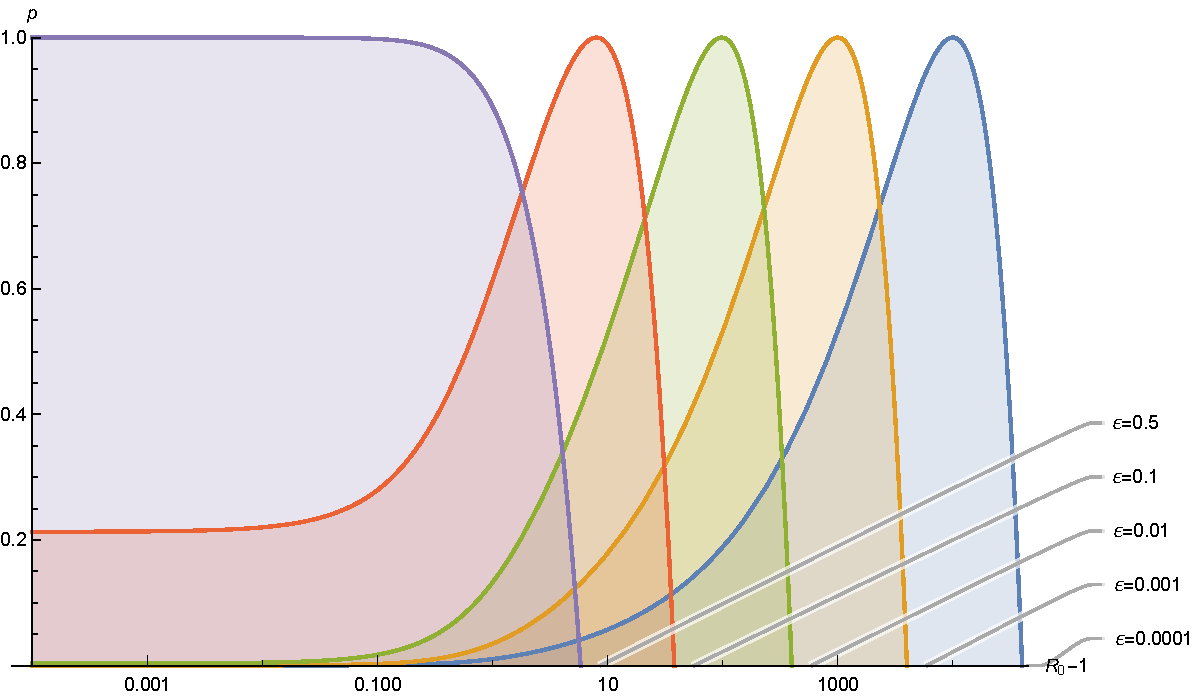
\includegraphics[width=0.9\textwidth]{Figures/Epsilons.pdf}
  \caption{The areas under each curves, which are shaded in different color, represent the region of damped oscillations, with respect to different $\epsilon$ values.}
\end{figure}

\subsubsection{Region of $(\R_0,\epsilon)$ plane where there are damped
  oscillations (fixed $p$)}

Again, I made plots with different $p$ in increasing order, the shade area between the blue curve and the orange curve represent the region where the system has damped oscillation.
\paragraph{$p=0$}
\begin{figure}[H]
  \centering
  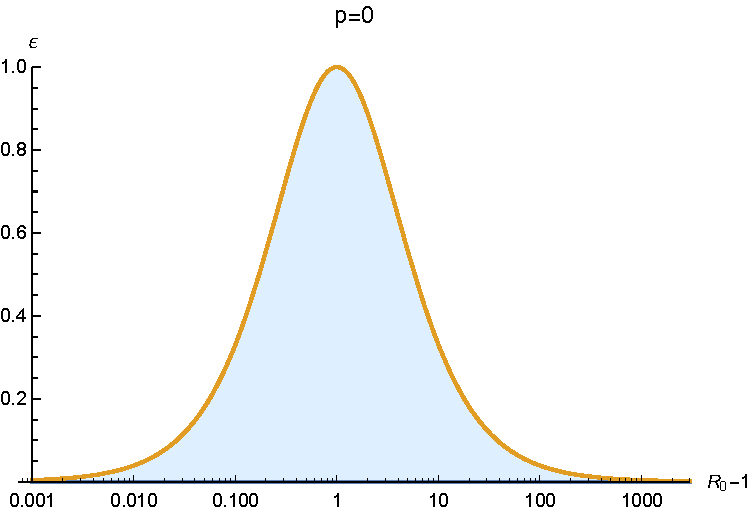
\includegraphics[width=1\textwidth]{Figures/p_0.pdf}
  \caption{$(\R_0,\epsilon)$ plane when $p=0$, damped oscillation occur at the shaded region below the orange curve.}
\end{figure}

\paragraph{$p=0.2$}
\begin{figure}[H]
  \centering
  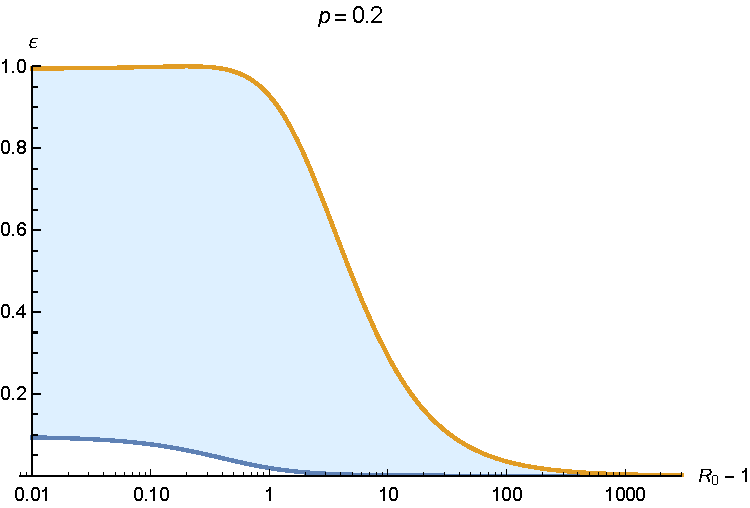
\includegraphics[width=1\textwidth]{Figures/p_0_2.pdf}
  \caption{$(\R_0,\epsilon)$ plane when $p=0.5$, damped oscillation occur at the shaded region between orange and blue curve.}
\end{figure}

\paragraph{$p=0.5$}
\begin{figure}[H]
  \centering
  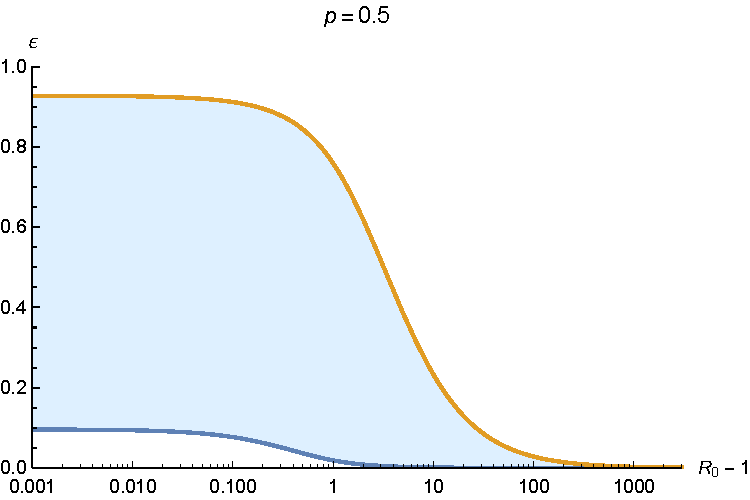
\includegraphics[width=1\textwidth]{Figures/p_0_5.pdf}
  \caption{$(\R_0,\epsilon)$ plane when $p=0.5$, damped oscillation occur at the shaded region between orange and blue curve.}
\end{figure}

\paragraph{$p=0.8$}
\begin{figure}[H]
  \centering
  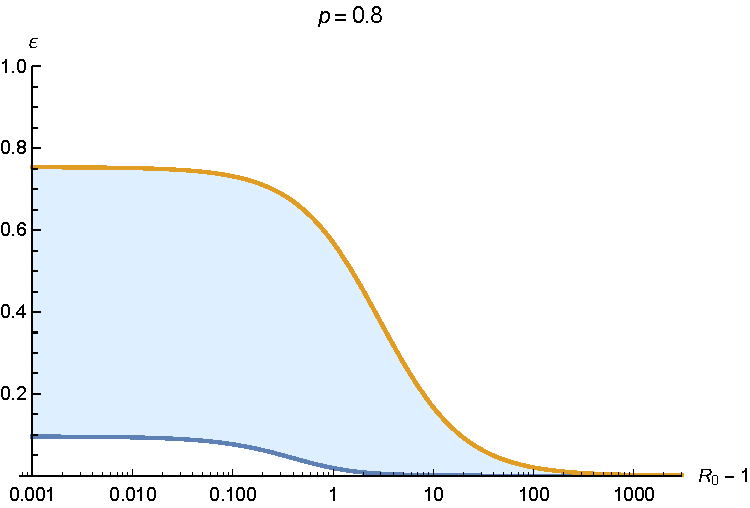
\includegraphics[width=1\textwidth]{Figures/p_0_8.pdf}
  \caption{$(\R_0,\epsilon)$ plane when $p=0.8$, damped oscillation occur at the shaded region between orange and blue curve.}
\end{figure}
\clearpage

\subsubsection{Comments and discussion on this model}
This is the initial model of intentional infection on newborns, which we obtained by directly modifying standard SIR model. Notice, the main difference between intentional infection model and vaccination model is the direction of flow of the individuals being treated with intentional infection/vaccination. Intentionally infected individuals are capable of transmitting the disease to susceptible individuals, whereas the vaccinated individuals will enter $R$(recovered) directly, therefore not able to impact the dynamics of the system anymore. 

In ideal cases, once an individual is intentionally infected, either directly or infected by others of the same kind, this individual will not be naturally infected anymore. Therefore, we should divide infected compartment into two separate infective classes, namely, intentionally infected and naturally infected.

In the past, for the case of smallpox, people believed that individuals that are variolated die much less often, compared with naturally infected cases. Here we define "advantageous" by fewer total death. More specifically, we would be comparing total disease induced mortality. Therefore, we need to involve a new parameter, namely, case fatality proportion.

\subsection{Model: Addition of disease induced mortality}\label{Newborn section}
\subsubsection{System of differential equations}
Disease induced mortality is created by deaths of infected population, with a certain ratio. The ratio is also known as case fatality proportion. 

Historic application of variolation have shown a lower case fatality proportion to those being variolated, compared to being naturally infected. Therefore, we need to assign different case fatality proportion to each classes. This also requires us to divide $I$ from our previous model into two distinct infective classes. Here, we call them "Intentionally infected" ($V$) and "Naturally infected" ($I$). 

In this model, we still assume no latent period, and similar to the last assumption in our previous model, we assume that all infected individuals(including $V$ and $I$) are equally infectious.

Therefore, our model becomes,
\begin{equation}\label{2}
\begin{split}
\dbyd{S}{t}&=\mu(1-p)- \beta S(V+I)-\mu S \,,\\
\dbyd{V}{t}&=\beta SV+\mu p-\gamma V -\mu V\,,\\
\dbyd{I}{t}&=\beta SI-\gamma I -\mu I\,,\\
\dbyd{M}{t}&=\pmV\gamma V+\pmI\gamma I\,,\\
\dbyd{R}{t}&=(1-\pmV)\gamma V+(1-\pmI)\gamma I-\mu R\,.
\end{split}
\end{equation}

In addition to the previous model, $\pmV$ and $\pmI$ represent the case fatality proportion for intentionally infected and naturally infected cases, respectively.

Again, we non-dimensionalize \autoref{2} by time, by
\begin{equation}
\tau=(\gamma+\mu)t \,,
\end{equation}
which yields,
\begin{subequations}\label{eq:base_ODE}
\begin{align}
\dbyd{S}{\tau}&=\epsilon(1-p)- \R_0 S(V+I)-\epsilon S\,, \label{eq:13a}\\
\dbyd{V}{\tau}&=\R_0 SV+\epsilon p-V\,, \label{eq:13b}\\
\dbyd{I}{\tau}&=\R_0 SI-I\,, \label{eq:13c}\\
\dbyd{M}{\tau}&=\pmV(1-\epsilon) V+\pmI(1-\epsilon) I\,,\\
\dbyd{R}{\tau}&=(1-\pmV)(1-\epsilon) V+(1-\pmI)(1-\epsilon) I-\epsilon R\,,
\end{align}
\end{subequations}

\subsubsection{Equilibria}

By letting \autoref{eq:13a}, \autoref{eq:13b} and \autoref{eq:13c} equal to 0, we solve for solutions.

If $p=0$, meaning there is no intentional infection, our system reduces to the standard SIR model.

There are two equilibriums for the standard SIR model, an Endemic equilibrium,
\begin{subequations}
\begin{align}
\hat{S} &= \frac{1}{\R_0}\,,\\
\hat{V} &= 0\,,\\
\hat{I} &= \epsilon(1-\frac{1}{\R_0})\,.
\end{align}
\end{subequations}

And a disease free equilibrium(since both $\hat{V}$ and $\hat{I}$ are 0),
\begin{subequations}
\begin{align}
\hat{S} &= 1\,,\\
\hat{V} &= 0\,,\\
\hat{I} &= 0\,.
\end{align}
\end{subequations}

However, if $p\neq 0$, the equilibrium is,
\begin{subequations}
\begin{align}
\hat{S}&= \frac{1}{\R_0}-\frac{2p}{(\R_0 -1)+ \sqrt{(\R_0-1)^2+4\R_0
         p}}\,, \label{eq:3Shat}\\
\hat{V}&= \frac{\epsilon(\R_0 -1)+ \epsilon \sqrt{(\R_0-1)^2+4\R_0 p}}{2\R_0}\,, \label{eq:Vhat}\\
\hat{I}&=0\,. \label{eq:Ihat}
\end{align}
\end{subequations}

Since $\hat{V}\neq 0$, for any $p$ between 0 and 1, this equilibrium is not disease free. It follows that this equilibrium is the endemic equilibrium.

Stability analysis relies on Jacobian matrix, which is,
\begin{equation}
\mathcal{J} =
\begin{bmatrix}
    \ -\R_0 (V+I)-\epsilon       & -\R_0 S     &-\R_0 S\\
    \ \R_0 V       & \R_0 S-1    &0\\
    \ \R_0 I       &0     &\R_0 S-1\\
\end{bmatrix}\,.
\end{equation}

Eigenvalues of Jacobian are given as follow,
\begin{subequations}
\begin{align}
\lambda_1&=-1+\R_0 S \label{eq:3lambda1}\\
\lambda_2&=\frac{-1+\R_0 S-\epsilon-\R_0 V-\sqrt{(-1+\R_0 S-\epsilon-\R_0 V)^2-4(\R_0+\epsilon-\R_0 S\epsilon)}}{2} \label{eq:lambda2}\\
\lambda_3&=\frac{-1+\R_0 S-\epsilon-\R_0 V+\sqrt{(-1+\R_0 S-\epsilon-\R_0 V)^2-4(\R_0+\epsilon-\R_0 S\epsilon)}}{2}\label{eq:lambda3}
\end{align}
\end{subequations}

By using \autoref{eq:3Shat} and \autoref{eq:3lambda1}, we obtain
\begin{equation}
-1+\R_0 S = - \frac{2p\R_0}{(\R_0 -1)+ \sqrt{(\R_0-1)^2+4\R_0 p}}<0
\end{equation}
Therefore,
\begin{equation}
\Re(\lambda_1) =-1+\R_0 S<0\,,
\end{equation}
To determine the real part of $\lambda_2$ and $\lambda_3$, we need to determine the sign of the quantity under the square root. 

By using \autoref{eq:3Shat} again, we have
\begin{equation}
\R_0 S\epsilon<\epsilon\,,
\end{equation}

Therefore,
\begin{equation}
(\R_0+\epsilon-\R_0 S\epsilon)>\R_0 >0\,,
\end{equation}
which means, if the sign of the quantity under the square root is positive, we will have
\begin{equation}
\sqrt{(-1+\R_0 S-\epsilon-\R_0 V)^2-4(\R_0+\epsilon-\R_0 S\epsilon)}<|(-1+\R_0 S-\epsilon-\R_0 V)|
\end{equation}
Therefore, $\Re(\lambda_2)<\Re(\lambda_3)<0$.

Certainly, if the sign of the quantity under the square root is negative,
\begin{equation}
\Re(\lambda_2)=\Re(\lambda_3)=-1+\R_0 S-\epsilon-\R_0 V<0
\end{equation}

We are able to conclude that EE is stable.

\subsubsection{Effect of intentional infection on total mortality}

In epidemic analysis, one way of measuring whether a certain method is more advantageous than another is to compare the total disease induced mortality. 

We first take a look at the mortality rate at EE,
\begin{equation}
\dbyd{M}{\tau}|_{EE}=\pmV(1-\epsilon)V=\frac{\pmV(1-\epsilon)\epsilon(\R_0 -1)+ \pmV(1-\epsilon)\epsilon \sqrt{(\R_0-1)^2+4\R_0 p}}{2\R_0}\,, \label{eq:dMdt}
\end{equation}

An important observation is, at EE, mortality rate increases as $p$ increases. This tells us, in the long run, having a larger proportion of intentional infection is unwise, since it leads extra deaths.

In history, smallpox was present in human population long before variolation was invented. When variolation was introduced, the population was already near equilibrium, with no intentional infection($p=0$). We are interested in the scenario where intentional infection is introduced after the population is in equilibrium, with no intentional infection.

One of the questions we want to answer is how long does it take for our system to reach the new EE. In fact the system will only infinitely approach the equilibrium instead of reaching it, therefore we need to define a threshold, which mean, how close does it need to be away from the equilibrium, do we consider it being at the equilibrium.

Since the new equilibrium has $\hat{I}=0$, we define reaching equilibrium by $I\leq 1\times 10^{-6}$ (one in a million).

In fact, if the case fatality proportion for intentionally infected cases is 1\%, we can hardly observe any differences between different proportion of intentional infection. To help us observe the dynamics better, we assume intentional infection has a 20\% case fatality proportion.

by plotting, we obtain \autoref{figure:0.0001}, we can see that it takes shorter time to reach the new EE for a larger proportion of intentional infection.
\begin{figure}[h]
  \centering
  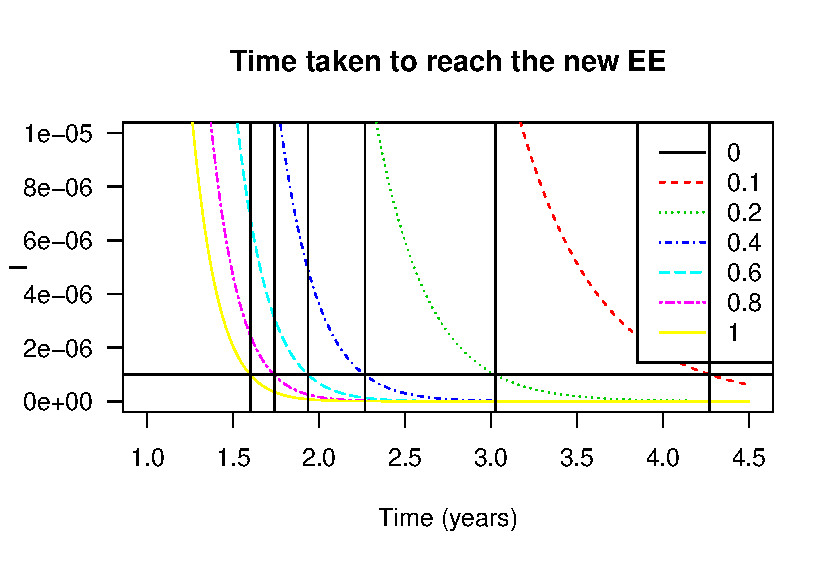
\includegraphics[width=0.9\textwidth]{Figures/I_less_than_0_000001.pdf}
  \caption{Determination of time taken to reach equilibrium}
\label{figure:0.0001}
\end{figure}

We are also interested in the time it takes for intentional infection to be more advantageous than non-intentional infection, by comparing total mortality.

From previous analysis, we learned that $\dbyd{M}{\tau}$ decreases over time, and stabilizes at a constant rate when reaching the new EE. But at the new EE, $\dbyd{M}{\tau}$ is higher when $p$ is higher. 

\begin{figure}[H]
  \centering
  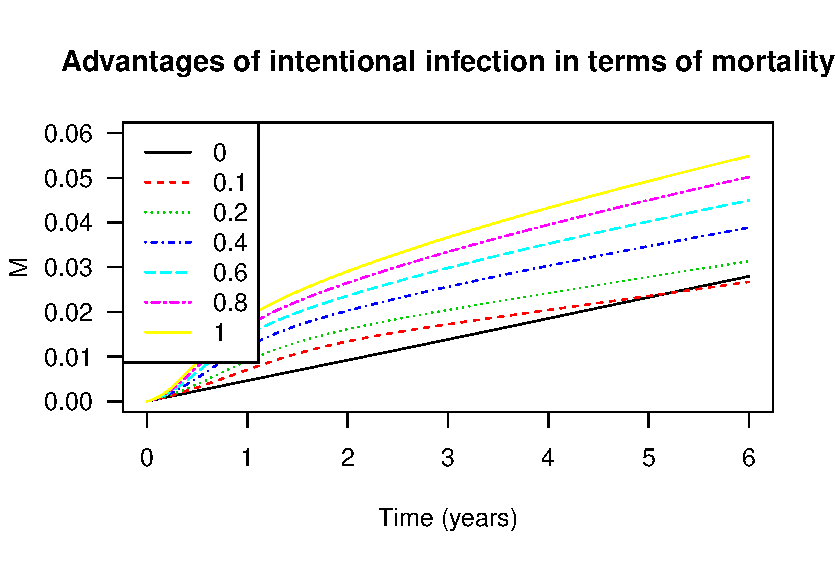
\includegraphics[width=0.9\textwidth]{Figures/dMdt.pdf}
  \caption{An illustration of intentional infection have advantages over non-intentional infection}
\label{figure:advantage}
\end{figure}

\autoref{figure:advantage} shows, at earlier times, intentional infections have steeper slopes than the black line, which is non-intentional infection. The slopes for intentional infection decreases over time, and eventually intentional infection with any proportion will have fewer total death than non-intentional infection.

\autoref{tab:times} summarize the times required to reach the new EE and time required to have advantages over non-intentional infection.

\begin{table}[H]
\begin{center}
\caption{Time required to reach equilibrium and have advantages over non-intentional infection}
\label{tab:times}
\smallskip
\begin{tabular}{c|c|r}
{\bfseries $p$} & {\bfseries Time to EE} & {\bfseries Time to have advantages} \\\hline
0.1 & 4.27 yrs & 5.20 yrs \\
0.2 & 3.03 yrs & 8.81 yrs \\
0.4 & 2.27 yrs & 17.45 yrs \\
0.6 & 1.94 yrs & 28.37 yrs \\
0.8 & 1.74 yrs & 42.43 yrs \\
1.0 & 1.60 yrs & 61.46 yrs
\end{tabular}
\end{center}
\end{table}
The table showed that as $p$ increases, the system reaches the new EE faster, but the time required to have advantages over non-intentional infection increase.

In fact, if $\pmV=0.01$, then the time required to have advantages over non-intentional infection is minimal, and the difference between different $p$ is also insignificant on a scale of years.

\begin{figure}[H]
  \centering
  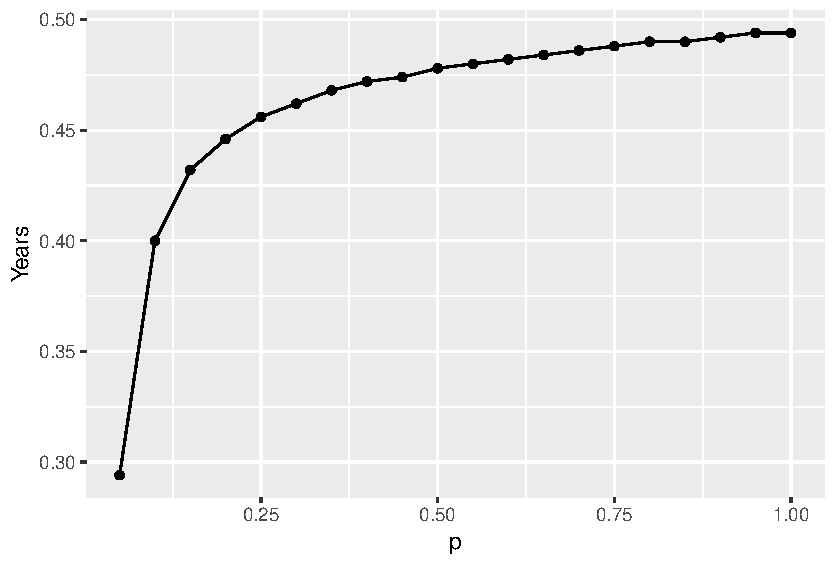
\includegraphics[width=0.9\textwidth]{Figures/Time_to_advantage_plot.pdf}
  \caption{Time to advantage, as a function of $p$}
\label{figure:advantage_by_p}
\end{figure}

\autoref{figure:advantage_by_p} shows us a relationship between time to advantage and $p$.

Here it shows, with a lower proportion of intentional infection, we gain advantage relatively faster. This conclusion is misleading, because it is suggesting that, with a minimal proportion of intentional infection, we can minimize the time it takes to gain advantage.

We found that, if $p$ is small, though it gains advantage faster, the number of deaths actually stays very close to non-intentional infection. In another word, the advantage is very insignificant.

Therefore, we want to suggest that, we can define a method being ``More advantageous'' than another to be: mortality by intentional infection is at least 10\% lower than mortality with no intentional infection.

\begin{figure}[H]
  \caption{Time for mortality of intentional infection is at least 10\% lower than non-intentional infection}\label{advantage2}
  \centering
  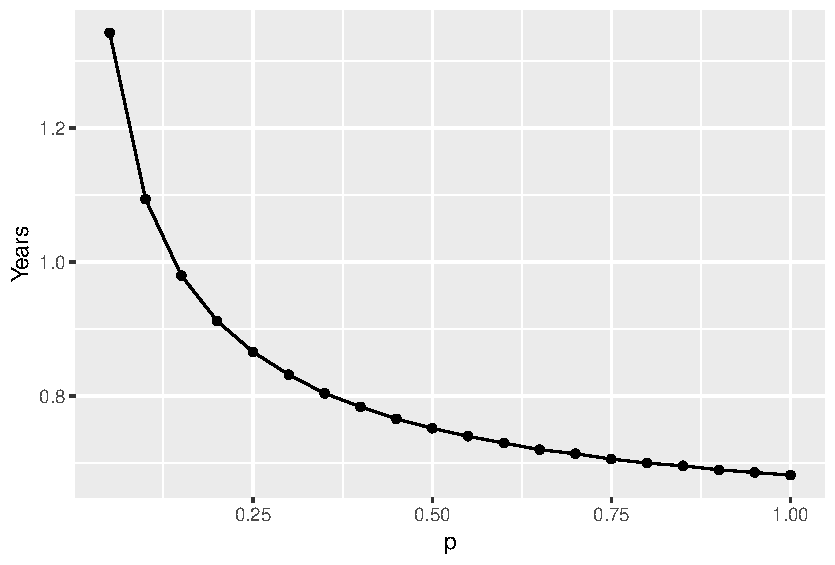
\includegraphics[width=1\textwidth]{Figures/New_time_to_advantage_plot.pdf}
\end{figure}
\autoref{advantage2} suggests, under our new definition of ``Have advantage'', the situation is reversed and larger proportion of intentional infection can be more advantageous relatively faster.

\subsubsection{Comments and discussion on this model}

In this model, we have shown that intentional infection has advantages over non-intentional infection in terms of total mortality. Which suggests, in history, the introduction of this technology does have positive effect on disease control, intuitively by reducing the number of deaths. However, interestingly, since a larger $p$ will lead to more death in the long run. Though a larger proportion of intentional infection can reduce total death and become more advantageous than non-intentional infection faster, it is unwise to keep infecting such a larger proportion of newborns. 

To summarize the above argument, if our strategy of intentional infection remain the same at all time, then in the long run, with a minimal proportion of intentional infection, total mortality could be minimized. However, in real life scenario, strategy does not need to be constant, it may be possible to intentionally infect at a relatively higher proportion initially, and decrease the proportion, or even stop intentional infection, with a combination of strategies like that, we could possibly minimize the total mortality. Or even eradicate the disease.

Other than strategic evolvement, there could still be some development to the model itself to make it more suitable to a realistic scenario. Since Intentional infection has a lower death rate, we could assume a milder symptom for intentionally infected cases. As a result, since aggressive symptoms are typical routes of disease transmission, lack of such pathways will lead to a decrease of transmission rate. Besides, intentionally and naturally infected cases could have different recovery rate. Therefore, our next model could consider various possibilities of these parameters, and draw conclusions to its behavior.

\subsubsection{Possibility of eradication}
If we define the disease been eradicated if the proportion of infected is less than one in a million. Then, our model is able to predict possible eradication of the disease.

At EE, $I=0$, although $I$ is going to approach 0 asymptotically, it will never completely cease to exist. However, we know that there is a point in forward time where $I<1\times10^{-6}$. Therefore, we can claim that naturally infected cases could be eradicated(we will show an example in the next section).

The next question would be whether it is possible for intentionally infected cases to burn out. After $I$ being wiped out, we could stop intentional infecting any other newborns. From then on if $S<\frac{1}{\R_0}$ for a long enough period of time, which means the effective $\R_0$ is less than 1, we could possibly observe $V<1\times10^{-6}$, which in return, represent the eradication of intentionally infected cases as well.

We use one example to illustrate the occurrence of such scenario. Assume we have $p=1$ until we reach EE. We could calculate $\hat{S}$ and $\hat{I}$. Now if we set the initial condition being the $\hat{S}$ and $\hat{I}$ we just calculated, and let $p=0$, we run the simulation and obtain the following,
\begin{figure}[H]
  \centering
  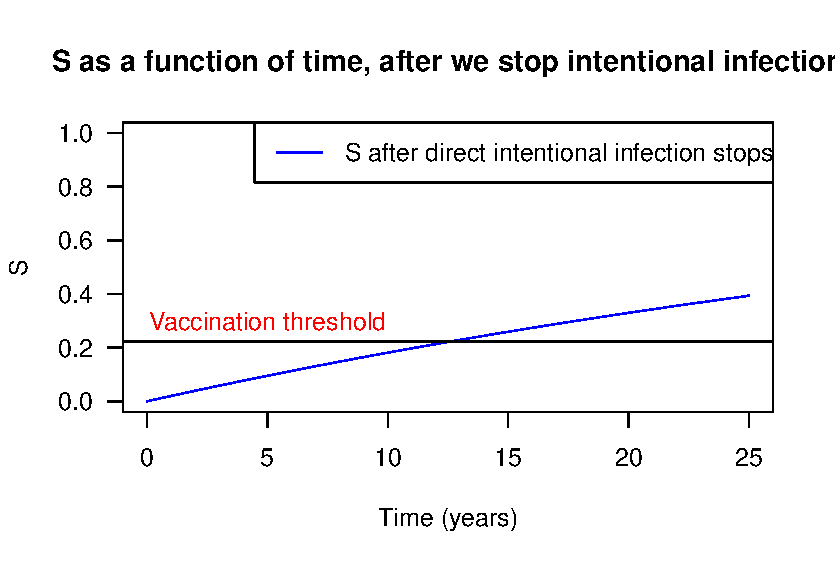
\includegraphics[width=1.1\textwidth]{Figures/Increase_of_S.pdf}
  \caption{For more than 10 years after we stop intentional infection, $S<\frac{1}{\R_0}$}
\label{figure:S_after_stop}
\end{figure}

\begin{figure}[H]
  \centering
  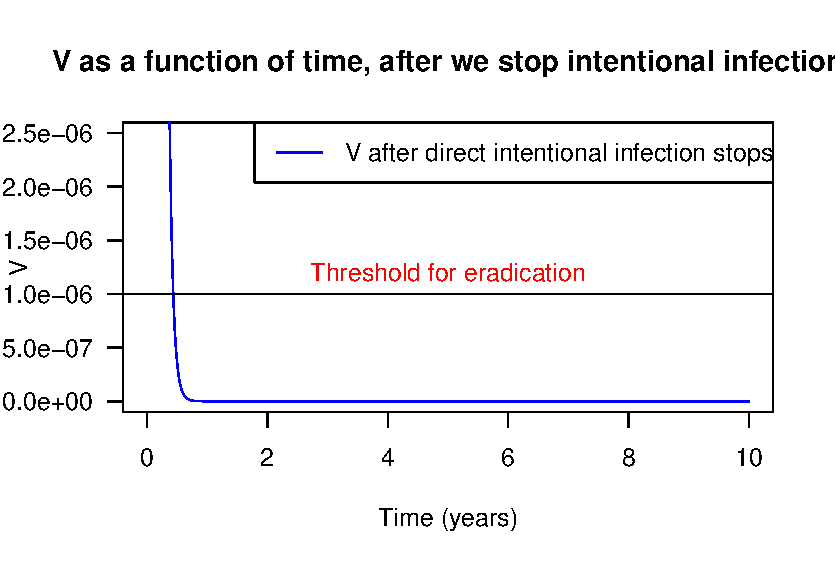
\includegraphics[width=1.1\textwidth]{Figures/V_after_stop.pdf}
  \caption{It takes less than 1 year for $V$ to fall below $1\times10^{-6}$}
\label{figure:V_after_stop}
\end{figure}

\autoref{figure:S_after_stop} and \autoref{figure:V_after_stop} have shown an example of disease eradication, by our definition. Other values of $p$ will still need to be investigated.

\subsection{Model: Different transmission rate and recovery rate}
\subsubsection{System of differential equations}
As we mentioned above, we need to involve new parameters for different transmission and recovery rate. Here, we let $\beta_V$ and $\beta_I$ represent the transmission rate of variolated cases and pathogen infected cases, respectively. $\gamma_V$ and $\gamma_I$ are the recovery rate of variolated cases and pathogen infected cases, respectively.

With the new parameters in hand, we now setup our system of differential equation,
\begin{equation}\label{model:complex}
\begin{split}
\dbyd{S}{t}&=\mu(1-p)- \beta_V SV -\beta_I SI-\mu S \,,\\
\dbyd{V}{t}&=\beta_V SV+\mu p-\gamma_V V -\mu V\,,\\
\dbyd{I}{t}&=\beta_I SI-\gamma_I I -\mu I\,,\\
\dbyd{M}{t}&=\pmV\gamma_V V+\pmI\gamma_I I\,,\\
\dbyd{R}{t}&=(1-\pmV)\gamma_V V+(1-\pmI)\gamma_I I-\mu R\,,
\end{split}
\end{equation}

We non-dimensionalize \autoref{model:complex} by scaling time, by
\begin{equation}
\tau=(\gamma_I+\mu)t \,,
\end{equation}

As the result, we obtain,
\begin{subequations}\label{eq:base_ODE}
\begin{align}
\dbyd{S}{\tau}&=\epsilon(1-p)-\R_{0,V} SV-\R_{0,I} SI-\epsilon S\,, \label{eq:S_by_tau}\\
\dbyd{V}{\tau}&=\R_{0,V} SV+\epsilon p-\tilde{\gamma} V\,, \label{eq:V_by_tau}\\
\dbyd{I}{\tau}&=\R_{0,I} SI-I\,, \label{eq:I_by_tau}\\
\dbyd{M}{\tau}&=\pmV(\tilde{\gamma}-\epsilon) V+\pmI(1-\epsilon) I\,,\\
\dbyd{R}{\tau}&=(1-\pmV)(\tilde{\gamma}-\epsilon) V+(1-\pmI)(1-\epsilon) I-\epsilon R\,,
\end{align}
\end{subequations}

Where $\R_{0,V}=\frac{\beta_V}{\gamma_I+\mu}$, $\R_{0,I}=\frac{\beta_I}{\gamma_I+\mu}$, $\tilde{\gamma}=\frac{\gamma_V+\mu}{\gamma_I+\mu}$, $\epsilon=\frac{\mu}{\gamma_I+\mu}$.

\subsubsection{Equilibria}

To solve for all equilibria, we let equations \autoref{eq:S_by_tau}, \autoref{eq:V_by_tau} and \autoref{eq:I_by_tau} equal to 0, we solve for solutions.

We acquired three sets of solutions. However, given conditions that all $\hat{S}$, $\hat{V}$ and $\hat{I}$ have to be a non-negative number between 0 and 1, we can discard two of the solutions, and the only set of solution left is, 
\begin{subequations}
\begin{align}
\hat{S}&= \frac{\R_{0,V}+\tilde{\gamma}-\sqrt{\R_{0,V}^2-2\R_{0,V}\tilde{\gamma}+\tilde{\gamma}^2+4p\R_{0,V}\tilde{\gamma}}}{2\R_{0,V}}\,, \label{eq:Shat}\\
\hat{V}&= \frac{\epsilon-\frac{\tilde{\gamma}\epsilon}{\R_{0,V}}+\frac{\epsilon\sqrt{\R_{0,V}^2-2\R_{0,V}\tilde{\gamma}+\tilde{\gamma}^2+4p\R_{0,V}\tilde{\gamma}}}{\R_{0,V}}}{2\tilde{\gamma}}\,, \label{eq:Vhat}\\
\hat{I}&=0\,, \label{eq:Ihat}
\end{align}
\end{subequations}

Similar to our previous models, since infected population at equilibrium is non-zero, this is not a disease free equilibrium but rather an endemic equilibrium.

Stability analysis rely on Jacobian Matrix,
\begin{equation}
\mathcal{J} =
\begin{bmatrix}
    \ -\R_{0,V}V-\R_{0,I}I-\epsilon       & -\R_{0,V}S     &-\R_{0,I}S\\
    \ \R_{0,V}V       & \R_{0,V}S-\gamma    &0\\
    \ \R_{0,I}I       &0     &\R_{0,I} S-1\\
\end{bmatrix}\,.
\end{equation}

Eigenvalues of Jacobian are given as follow,
\begin{subequations}
\begin{align}
\lambda_1&=-1+\R_{0,I} S \label{eq:lambda1}\\
\lambda_2&=\frac{-\tilde{\gamma}+\R_{0,V}S-\epsilon-\R_{0,V}V-\sqrt{(-\tilde{\gamma}+\R_{0,V} S-\epsilon-\R_{0,V}V)^2-4(\R_{0,V}\tilde{\gamma}+\epsilon\tilde{\gamma}-\R_{0,V}S\epsilon)}}{2} \label{eq:lambda2}\\
\lambda_3&=\frac{-\tilde{\gamma}+\R_{0,V}S-\epsilon-\R_{0,V}V+\sqrt{(-\tilde{\gamma}+\R_{0,V} S-\epsilon-\R_{0,V}V)^2-4(\R_{0,V}\tilde{\gamma}+\epsilon\tilde{\gamma}-\R_{0,V}S\epsilon)}}{2}\label{eq:lambda3}
\end{align}
\end{subequations}

By using \autoref{eq:Shat}, we know that
\begin{equation}
0\leq S\leq \frac{\tilde{\gamma}}{\R_{0,V}}\,.{\label{middle}}
\end{equation}
Therefore, 
\begin{equation}
\Re(\lambda_1) <0
\end{equation}
iff 
\begin{equation}
\frac{\tilde{\gamma}}{\R_{0,V}}<\frac{1}{\R_{0,I}}
\end{equation}

Or equivalently 
\begin{equation}
\frac{\beta_V}{\beta_I}<\tilde{\gamma}^2
\end{equation}
Intuitively, if recovery rate are similar for variolated and normally infected cases, i.e. $\tilde{\gamma}\approx 1$, the endemic equilibrium is unstable if $\R_{0,V}<\R_{0,I}$

For the real part of $\lambda_2$ and $\lambda_3$, first we look at the terms before square root. 

By using \autoref{middle}, we have
\begin{equation}
-\tilde{\gamma}+\R_{0,V}S-\epsilon-\R_{0,V}V<0\,,
\end{equation}

Therefore,
\begin{equation}
\Re(\lambda_2)<-\tilde{\gamma}+\R_{0,V}S-\epsilon-\R_{0,V}V<0\,,
\end{equation}

Next, notice
\begin{equation}
\R_{0,V}\tilde{\gamma}+\epsilon\tilde{\gamma}-\R_{0,V}S\epsilon>0\,.
\end{equation}
It follows that
\begin{equation}
\sqrt{(-\tilde{\gamma}+\R_{0,V} S-\epsilon-\R_{0,V}V)^2-4(\R_{0,V}\tilde{\gamma}+\epsilon\tilde{\gamma}-\R_{0,V}S\epsilon)}<|-\tilde{\gamma}+\R_{0,V} S-\epsilon-\R_{0,V}V|
\end{equation}
Therefore, $\Re(\lambda_3)<0$.

As a result, we cannot directly conclude the stability of EE, but we have observed that stability depends on $\tilde{\gamma}$ and $\R_{0,I}$

\subsubsection{Comments and discussion on this model}

Parameters of this model such as $\R_{0,V}$ and $\gamma_V$ are custom to the design of pathogen used for intentional infection. 

Previous study have shown that, for a similar model which does not consider death, a significant decrease in final size is expected, for a transmissible vaccine, even when $\R_{0,V}$ is less than 1, e.g. $\R_{0,V}=0.5$, we would expect similar results for our model, the difference is, with the addition of birth and death rate, since our system have shown that the disease cannot be completely eradicated, there will always be newly infected cases, therefore, we do not have a final size estimation. 

\section{Model: Intentionally infect susceptible with a certain rate}
\subsection{Model: Modification to SIR model}
\subsubsection{System of differential equations}
Our second strategy is to intentionally infect susceptible individuals with a certain rate. Again, we start our analysis by modifying the standard SIR model.

The following assumptions are made:
\begin{itemize}
\item No disease induced mortality.
\item Birth and natural death rate are the same, the total population remains constant.
\item Latent period is short enough to be ignored.
\item All susceptible individuals are equally likely to be infected, and all infected individuals are equally infectious.
\end{itemize}

\begin{equation}\label{1}
\begin{split}
\dbyd{S}{t}&=\mu- \beta SI-rS-\mu S\,, \\
\dbyd{I}{t}&=rS+\beta SI-\gamma I -\mu I\,,\\
\dbyd{R}{t}&=\gamma I-\mu R\,.
\end{split}
\end{equation}

Here, $\beta$ is transmission rate, $\gamma$ is recovery rate, $\mu$ is the \emph{per capita} rate of birth and death, $r$ is the rate of intensional infection on susceptible individuals. We will discuss the reasonable value of $r$ in later sections.

We convert our system into dimensionless form, by scaling time, by

\begin{equation}
\tau=(\gamma+\mu)t\,.
\end{equation}

Therefore, the dimensionless system is:
\begin{equation}
\begin{split}
\dbyd{S}{\tau}&=\epsilon- \R_0  SI-\eta S-\epsilon S\,, \\
\dbyd{I}{\tau}&=\eta S+\R_0 SI-I\,,\\
\dbyd{R}{\tau}&=(1-\epsilon)I-\epsilon R\,,
\end{split}
\end{equation}

where $\epsilon=\frac{\mu}{\gamma+\mu}$, $\R_0=\frac{\beta}{\gamma+\mu}$, $\eta=\frac{r}{\gamma+\mu}$

\subsubsection{Equilibrium}
We obtain only one solution by solving the system:
\begin{subequations}
\begin{align}
\hat{S} &= \frac{1}{\R_0}-\frac{2\eta}{\R_0(-(\eta+\epsilon-\epsilon\R_0)+\sqrt{(\eta+\epsilon-\epsilon\R_0)^2+4\R_0\epsilon \eta}+2\eta)}\\
\hat{I} &= \frac{-(\eta+\epsilon-\epsilon\R_0)+\sqrt{(\eta+\epsilon-\epsilon\R_0)^2+4\R_0\epsilon \eta}}{2\R_0}
\end{align}
\end{subequations}
Notice, for any non-zero $\eta$, $\hat{I}\neq 0$, it follows that this equilibrium is also an endemic equilibrium, since there is always proportion of population that are infected.

Stability analysis rely on Jacobian matrix, which is,
\begin{equation}
\mathcal{J} =
\begin{bmatrix}
    \ -\R_0 I-\eta-\epsilon       & -\R_0 S \\
    \ \eta+\R_0 I       & \R_0 S-1 \\
\end{bmatrix}\,.
\end{equation}

For simplicity. Let 
\begin{equation}
G=-(\eta+\epsilon-\epsilon\R_0)+\sqrt{(\eta+\epsilon-\epsilon\R_0)^2+4\R_0\epsilon \eta}.
\end{equation}
Notice, if $\epsilon,\eta\neq 0$, $G>0$. 

So Jacobian at EE becomes,
\begin{equation}
\mathcal{J}|_{E.E.}=
\begin{bmatrix}
    \ \frac{G}{2}-\eta-\epsilon       & -1+\frac{2\eta}{G+2\eta} \\
    \ \eta+\frac{G}{2}       & -\frac{2\eta}{G+2\eta} \\
\end{bmatrix}\,.
\end{equation}

The eigenvalues of of Jacobian are:

\begin{align}
\lambda_{1,2} &= \frac{-(G^2+4\eta G+2\epsilon G+4\eta^2+4\epsilon\eta+4\eta) }{4(G+2\eta)}\\
& \pm \frac{\sqrt{((G^2+4\eta G+2\epsilon G+4\eta^2+4\epsilon\eta+4\eta)^2-4(2G^3+12\eta G^2+24\eta^2 G+8\epsilon\eta G+16\eta^3+16\epsilon\eta^2)}}{4(G+2\eta)}
\end{align}

We know that $G>0$, and since the rate of intentional infection is non-zero, so $\eta >0$

Since we are only interested in the case where the rate of intentional infection is non-zero, we assume that $\eta>0$. Together with the fact that $G>0$, the discriminant($\Delta$) satisfies the following inequality,
\begin{equation}
\Delta<|(G^2+4\eta G+2\epsilon G+4\eta^2+4\epsilon\eta+4\eta)|
\end{equation}

Therefore, we can conclude that Re($\lambda$)$<0$, which means, EE is stable.

To fully understand the dynamics of the system, we want to know whether or not there is a damped oscillation. This is done by determining the sign of the discriminant.

We will start our analysis with specific values of each parameter. Again, we will use parameters of smallpox. The values are listed in \autoref{tab:params}.
\subsubsection{Region of ($\R_0$,$\eta$) plane where there are damped oscillations (fixed $\epsilon$)}

$\eta$ is the rate of intentional infection, $\R_0$ is the basic reproduction number.
\begin{figure}[H]
  \centering
  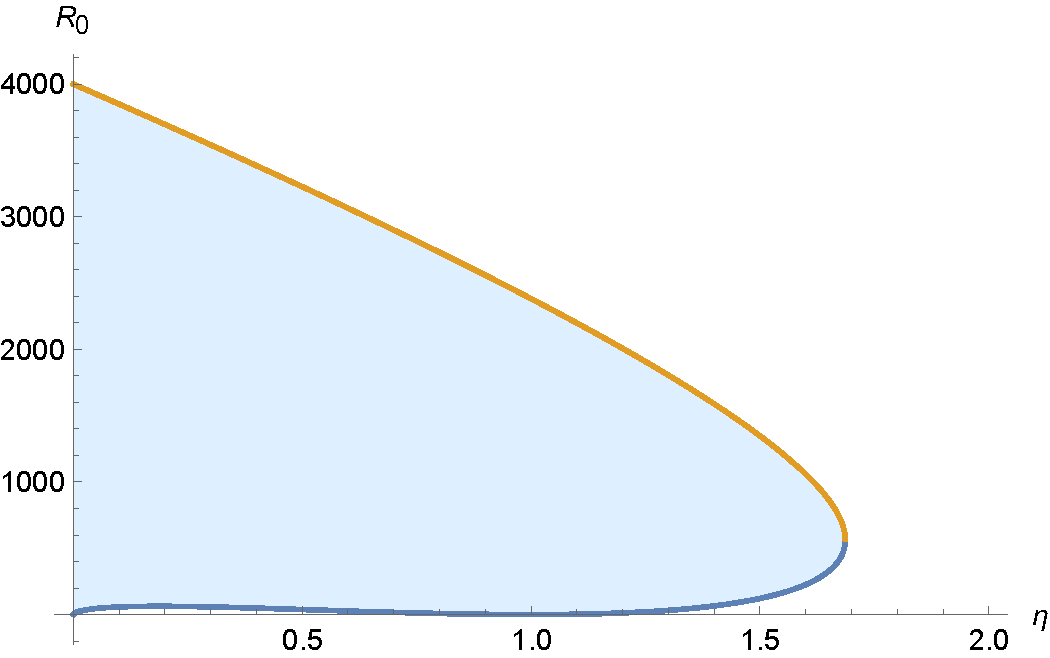
\includegraphics[width=1\textwidth]{Figures/sus0_001.pdf}
  \caption{The graph shows the ($\R_0,\eta$ plane) when $\epsilon=0.001$. The shaded region is where there is going to be damped oscillations}
\end{figure}

\begin{figure}[H]
  \centering
  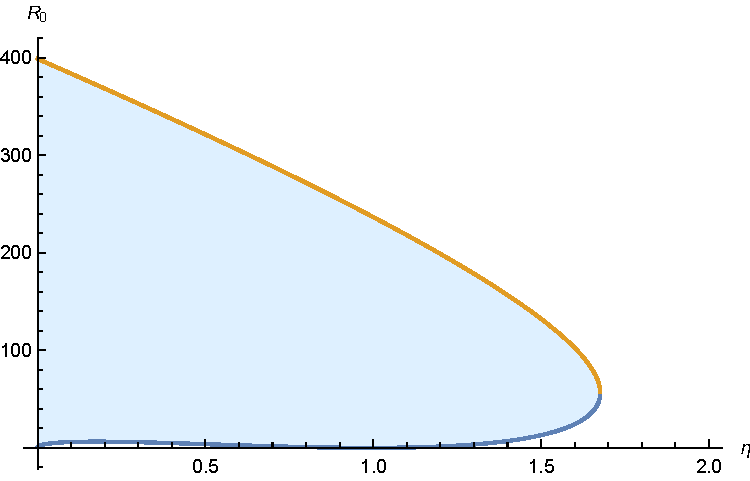
\includegraphics[width=1\textwidth]{Figures/sus0_01.pdf}
  \caption{The graph shows the ($\R_0,\eta$ plane) when $\epsilon=0.01$. The shaded region is where there is going to be damped oscillations}
\end{figure}

\begin{figure}[H]
  \centering
  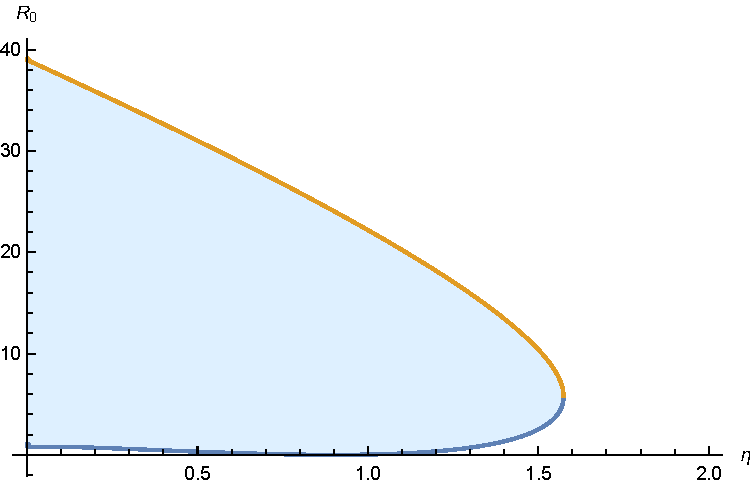
\includegraphics[width=1\textwidth]{Figures/sus0_1.pdf}
  \caption{The graph shows the ($\R_0,\eta$ plane) when $\epsilon=0.1$. The shaded region is where there is going to be damped oscillations}
\end{figure}

\begin{figure}[H]
  \centering
  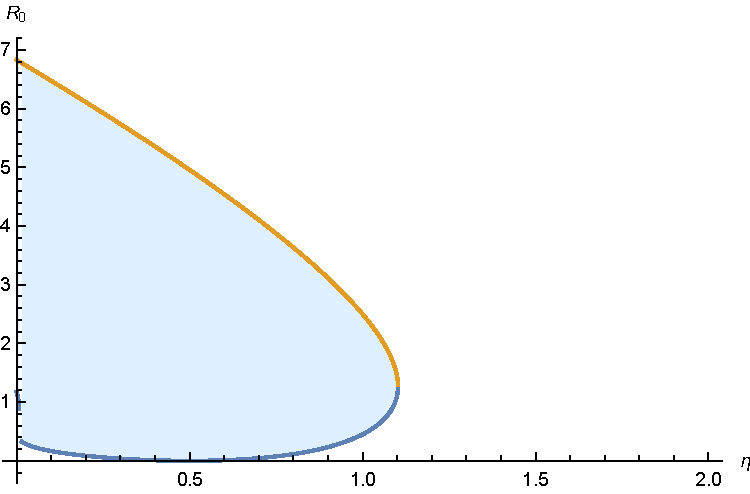
\includegraphics[width=1\textwidth]{Figures/sus0_5.pdf}
  \caption{The graph shows the ($\R_0,\eta$ plane) when $\epsilon=0.5$. The shaded region is where there is going to be damped oscillations}
\end{figure}

\subsubsection{Comments and discussion on this model}
Similar to our newborn infection model, the model obtained by modifying the standard SIR model is rather simple. We will still need to divide the infected compartment into intentionally and naturally infected classes.

Furthermore, to help us conclude whether or not there is any positive effect by intentionally infecting, we will need to involve disease induced mortality. This may also help us compare two different strategies of intentional infection.

\subsection{Model: Addition of disease induced mortality}

\subsubsection{System of differential equations}

The addition of disease induced mortality will require the involvement of case fatality proportion, again. 

Here, we are doing exactly the same adjustment as we did in \autoref{Newborn section}.
Our new system is,

\begin{subequations}\label{1}
\begin{align}
\dbyd{S}{t}&=\mu- \beta S(V+I)-rS-\mu S \,,\\
\dbyd{V}{t}&=\beta SV+rS-\gamma V -\mu V\,,\\
\dbyd{I}{t}&=\beta SI-\gamma I -\mu I\,,\\
\dbyd{M}{t}&=\pmV\gamma V+\pmI\gamma I\,,\\
\dbyd{R}{t}&=(1-\pmV)\gamma V+(1-\pmI)\gamma I-\mu R\,,
\end{align}
\end{subequations}

where $\beta$ is transmission rate, $\gamma$ is recovery rate, $\mu$ is the \emph{per capita} rate of birth and death, $r$ is the rate of intensional infection on susceptible individuals.

We non-dimensionalize \autoref{1} by scaling time, by
\begin{equation}
\tau=(\gamma+\mu)t \,,
\end{equation}

As the result, we obtain,

\begin{subequations}\label{eq:base}
\begin{align}
\dbyd{S}{\tau}&=\epsilon-\eta S-\R_0 S(V+I)-\epsilon S\,, \label{3a}\\
\dbyd{V}{\tau}&=\R_0 SV+\eta S-V\,, \label{3b}\\
\dbyd{I}{\tau}&=\R_0 SI-I\,, \label{3c}\\
\dbyd{M}{\tau}&=\pmV(1-\epsilon) V+\pmI(1-\epsilon) I\,,\\
\dbyd{R}{\tau}&=(1-\pmV)(1-\epsilon) V+(1-\pmI)(1-\epsilon) I-\epsilon R\,,
\end{align}
\end{subequations}

Where $\epsilon=\frac{\mu}{\gamma+\mu}$, $\R_0=\frac{\beta}{\gamma+\mu}$, $\eta=\frac{r}{\gamma+\mu}$

\subsubsection{Equilibria}
If $\eta=0$, the system will again be simplified to the standard SIR model, the equilibrium of that has been shown before. Here, we are only interested in the case where $\eta\neq0$.

The only solution we obtain by solving the system is:

\begin{subequations}\label{eq:EE}
\begin{align}
\hat{S} &= \frac{1}{\R_0}-\frac{2\eta}{\R_0(-(\eta+\epsilon-\epsilon\R_0)+\sqrt{(\eta+\epsilon-\epsilon\R_0)^2+4\R_0\epsilon \eta}+2\eta)}\,, \label{eq:Shat}\\
\hat{V} &= \frac{-(\eta+\epsilon-\epsilon\R_0)+\sqrt{(\eta+\epsilon-\epsilon\R_0)^2+4\R_0\epsilon \eta}}{2\R_0}\,, \label{eq:Vhat}\\
\hat{I} &= 0\,,
\end{align}
\end{subequations}

Notice, $\hat{V}$ is non-zero, therefore this equilibrium is not a disease free equilibrium. It follows that it is the endemic equilibrium.

\subsubsection{Stability of Endemic Equilibrium}

The Jacobian matrix of this system is,
\begin{equation}
\mathcal{J} =
\begin{bmatrix}
    \ -\eta-\R_0 (V+I)-\epsilon       & -\R_0 S     &-\R_0 S\\
    \ \R_0 V+\eta       & \R_0 S-1    &0\\
    \ \R_0 I       &0     &\R_0 S-1\\
\end{bmatrix}\,.
\end{equation}

Eigenvalues of Jacobian are ,
\begin{subequations}
\begin{align}
\lambda_1&=-1+\R_0 S \label{eq:lambda1}\\
\lambda_2&=\frac{-1+\R_0 S-\eta-\epsilon-\R_0 V+\sqrt{(-1+\R_0 S-\eta-\epsilon-\R_0 V)^2-4(\eta+\R_0 V+\epsilon-\R_0 S\epsilon)}}{2}\\
\lambda_3&=\frac{-1+\R_0 S-\eta-\epsilon-\R_0 V-\sqrt{(-1+\R_0 S-\eta-\epsilon-\R_0 V)^2-4(\eta+\R_0 V+\epsilon-\R_0 S\epsilon)}}{2}
\end{align}
\end{subequations}

By using \autoref{eq:Shat} and \autoref{eq:lambda1}, we get
\begin{equation}
\Re(\lambda_1)=-1+\R_0 S=-\frac{2\eta}{(-(\eta+\epsilon-\epsilon\R_0)+\sqrt{(\eta+\epsilon-\epsilon\R_0)^2+4\R_0\epsilon \eta}+2\eta)}<0
\end{equation}

To decide the real parts of $\lambda_2$ and $\lambda_3$, we need to determine the sign of the quantity under the square root.

By using \autoref{eq:Shat} again, we have
\begin{equation}
\R_0 S\epsilon<\epsilon\,,
\end{equation}

Therefore
\begin{equation}
(\eta+\R_0 V+\epsilon-\R_0 S\epsilon)>0\,,
\end{equation}

It follows that
\begin{equation}
\sqrt{(-1+\R_0 S-\eta-\epsilon-\R_0 V)^2-4(\eta+\R_0 V+\epsilon-\R_0 S\epsilon)}<|(-1+\R_0 S-\eta-\epsilon-\R_0 V)|\,.
\end{equation}

It follows that we have two cases, if the quantity under square root is negative, then
\begin{equation}
\Re(\lambda_2)=\Re(\lambda_3)=-1+\R_0 S-\eta-\epsilon-\R_0 V<0\,,
\end{equation}

Otherwise, we have
\begin{equation}
\Re(\lambda_3)<\Re(\lambda_2)<0
\end{equation}

We are able to conclude that EE is stable.

\subsubsection{The effect of intentional infection on mortality}
We will again start by looking at the mortality rate at EE.

By using \autoref{eq:base} and \autoref{eq:Vhat}, we can find the mortality rate at EE,
\begin{equation}
\dbyd{M}{\tau}=\pmV(1-\epsilon)V=\frac{\pmV(1-\epsilon)\epsilon(\R_0 -1)+ \pmV(1-\epsilon)\epsilon \sqrt{(\R_0-1)^2+4\R_0 p}}{2\R_0}\,, \label{eq:dMdt}
\end{equation}
as shown the following graph,
\begin{figure}[H]
  \centering
  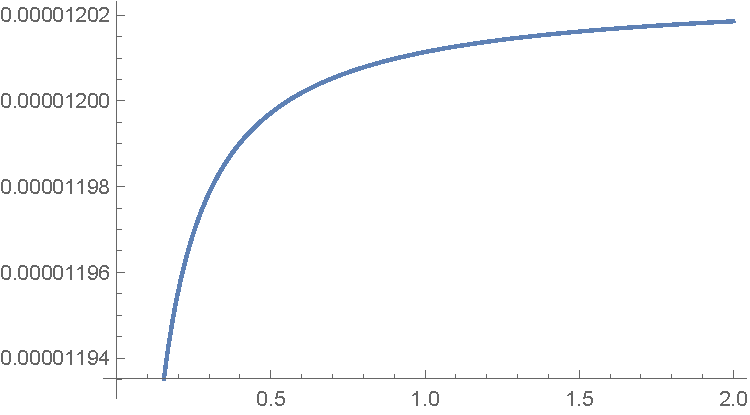
\includegraphics[width=1\textwidth]{Figures/M_at_EE.pdf}
  \caption{$\dbyd{M}{\tau}$ at EE as a function of $\eta$.}
\end{figure}

It is worthwhile noticing that, as we increase the rate of intentional infection, the mortality rate eventually reaches an asymptote at around $1.2\times10^{-5}$, which is very close to the mortality rate when we intentionally infect newborn individuals with a highest proportion ($p=1$). This suggests, in the long run, a high proportion of newborn infection would have similar result as intentionally infect susceptible at a high rate.

As we did in newborn model, we also want to know the time it takes for susceptible intentional infection to reach the new equilibrium, as well as the time it takes to be advantageous over non-intentional infection.

\begin{figure}[H]
  \centering
  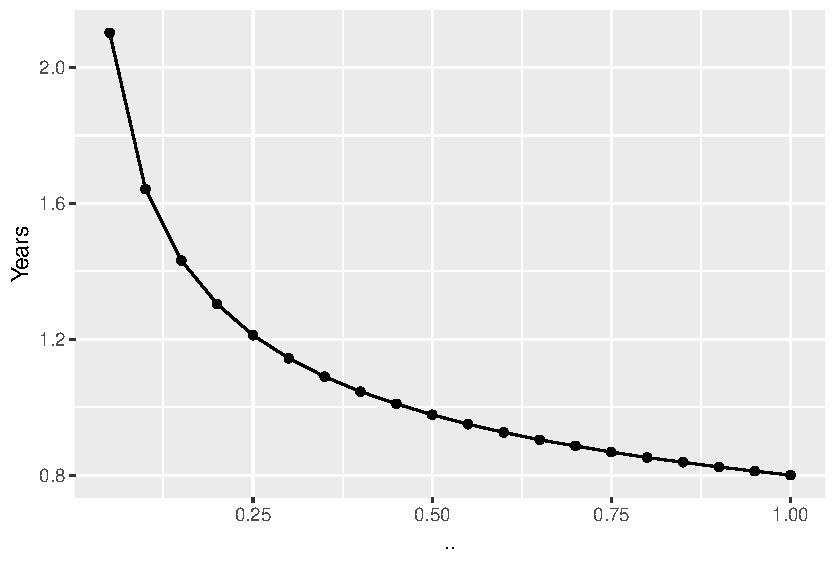
\includegraphics[width=1\textwidth]{Figures/Susceptible_Equilibrium.pdf}
  \caption{Time taken for susceptible intentional infection to reach the new equilibrium}
\end{figure}

\begin{figure}[H]
  \centering
  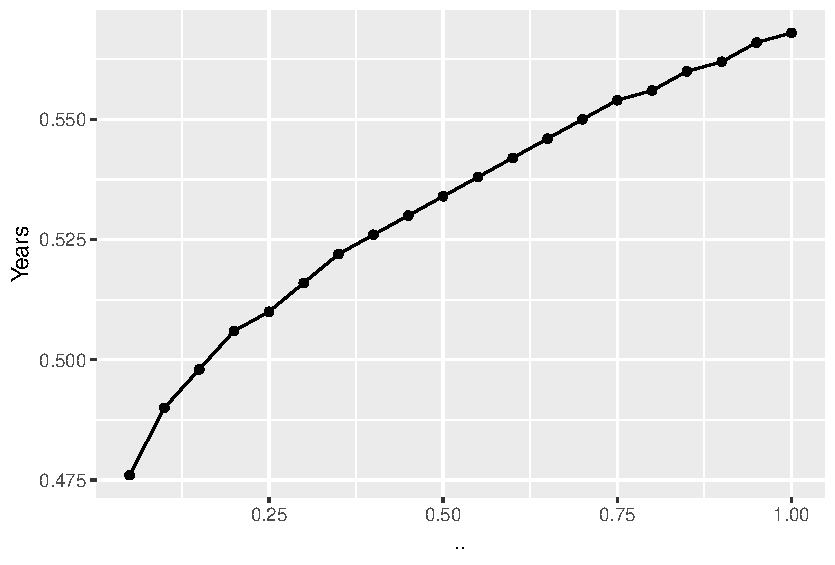
\includegraphics[width=1\textwidth]{Figures/Susceptible_advantageous.pdf}
  \caption{Time taken for susceptible intentional infection to have at least 10$\%$ fewer disease induced mortality.}
\end{figure}

Unlike the newborn infection model, in this scenario, the time required for intentional infection to be more advantageous increases as the rate of intentional infection increases. This is suggesting, with a minimal rate of intentional infection, not only can long term mortality be at minimum, but also able to be advantageous relative faster.
\subsubsection{Comments and discussion to this model}
We have proven the benefit of intentional infection on susceptible individuals. With any rate of intentional infection, we can always reduce the disease induced mortality. As we discussed in the previous section, we cannot conclude an optimal rate of intentional infection, since we have shown that the benefit is maximized, in every aspect, when the rate of intentional infection is minimal. Further study is required to answer this question.
\section{Conclusion}
Since our models include birth and natural death, we are essentially having infinite populations, which also means, the disease induced mortality will also be infinite. For that reason, we are unable to compare these two different strategies directly.

Nevertheless however, we have shown that both strategies can bring us benefit in the long run. Though may not be able to completely eradicate the disease, but at least greatly reduce disease induced mortalities, in the case of smallpox, death.

Due to existence of special events or accidents happening in real life, which can alter the situation of disease spread, we have many different factor not being considered in our models. For both strategies, the models can still be modified and developed to higher complexity. For example, smallpox variolation is done via skin. However, since the subject used to variolate is live smallpox virus, there could be some other pathways for such virus to enter respiratory system. An example of such a pathway could be scratching the area of variolation followed by touching nose.

In such scenario, though the individual infected via skin might have symptoms much less severe than naturally infection, when the virus happens to enter respiratory system, a natural infection could still occur. The result of that will be the individual entering naturally infected class.

We do not have enough sources to conclude the likelihood of such incidence, therefore not able to conclude whether or not this could affect our systems and conclusions.
\section{Future work}
This section elaborates some ideas for future use and needs to be investigated later.
\begin{itemize}
\item Comparison between intentional infection and traditional vaccine, which does not transmit. This is for showing intentional infection as a more effective method to vaccinate.
\item We can use our model to see how well they fit the historical data for smallpox. This could help us much better understand the variolation history of smallpox.
\end{itemize}

\end{document}
